\documentclass[10pt,a4paper,onecolumn]{article}
\usepackage{marginnote}
\usepackage{graphicx}
\usepackage[rgb,svgnames]{xcolor}
\usepackage{authblk,etoolbox}
\usepackage{titlesec}
\usepackage{calc}
\usepackage{tikz}
\usepackage[pdfa]{hyperref}
\usepackage{hyperxmp}
\hypersetup{%
    unicode=true,
    pdfapart=3,
    pdfaconformance=B,
    pdftitle={phrosty: A difference imaging pipeline for Roman},
    pdfauthor={Lauren N. Aldoroty, Lei Hu, Rob A. Knop, Cole Meldorf,
Daniel Scolnic, Shu Liu, W. Michael Wood-Vasey, Marcus Manos, Lucas
Erlandson, Rebekah Hounsell, Ben Rose, Masao Sako, Michael Troxel, The
Roman Supernova Cosmology Project Infrastructure Team},
    pdfpublication={Journal of Open Source Software},
    pdfpublisher={Open Journals},
    pdfissn={2475-9066},
    pdfpubtype={journal},
    pdfvolumenum={},
    pdfissuenum={},
    pdfdoi={10.xxxxxx/draft},
    pdfcopyright={Copyright (c) 1970, Lauren N. Aldoroty, Lei Hu, Rob A.
Knop, Cole Meldorf, Daniel Scolnic, Shu Liu, W. Michael Wood-Vasey,
Marcus Manos, Lucas Erlandson, Rebekah Hounsell, Ben Rose, Masao Sako,
Michael Troxel, The Roman Supernova Cosmology Project Infrastructure
Team},
    pdflicenseurl={http://creativecommons.org/licenses/by/4.0/},
    colorlinks=true,
    linkcolor=[rgb]{0.0, 0.5, 1.0},
    citecolor=Blue,
    urlcolor=[rgb]{0.0, 0.5, 1.0},
    breaklinks=true
}
% https://tex.stackexchange.com/a/535849
% Create an OutputIntent in order to correctly specify colours
\immediate\pdfobj stream attr{/N 3} file{sRGB.icc}
\pdfcatalog{%
  /OutputIntents [
    <<
      /Type /OutputIntent
      /S /GTS_PDFA1
      /DestOutputProfile \the\pdflastobj\space 0 R
      /OutputConditionIdentifier (sRGB)
      /Info (sRGB)
    >>
  ]
}
\pdfvariable omitcidset=1
\usepackage{caption}
\usepackage{orcidlink}
\usepackage{tcolorbox}
\usepackage{amssymb,amsmath}
\usepackage{ifxetex,ifluatex}
\usepackage{seqsplit}
\usepackage{xstring}

\usepackage{float}
\let\origfigure\figure
\let\endorigfigure\endfigure
\renewenvironment{figure}[1][2] {
    \expandafter\origfigure\expandafter[H]
} {
    \endorigfigure
}

\usepackage{fixltx2e} % provides \textsubscript

% definitions for citeproc citations
\NewDocumentCommand\citeproctext{}{}
\NewDocumentCommand\citeproc{mm}{%
  \begingroup\def\citeproctext{#2}\cite{#1}\endgroup}
\makeatletter
 % allow citations to break across lines
 \let\@cite@ofmt\@firstofone
 % avoid brackets around text for \cite:
 \def\@biblabel#1{}
 \def\@cite#1#2{{#1\if@tempswa , #2\fi}}
\makeatother
\newlength{\cslhangindent}
\setlength{\cslhangindent}{1.5em}
\newlength{\csllabelwidth}
\setlength{\csllabelwidth}{3em}
\newenvironment{CSLReferences}[2] % #1 hanging-indent, #2 entry-spacing
 {\begin{list}{}{%
  \setlength{\itemindent}{0pt}
  \setlength{\leftmargin}{0pt}
  \setlength{\parsep}{0pt}
  % turn on hanging indent if param 1 is 1
  \ifodd #1
   \setlength{\leftmargin}{\cslhangindent}
   \setlength{\itemindent}{-1\cslhangindent}
  \fi
  % set entry spacing
  \setlength{\itemsep}{#2\baselineskip}}}
 {\end{list}}
\usepackage{calc}
\newcommand{\CSLBlock}[1]{\hfill\break\parbox[t]{\linewidth}{\strut\ignorespaces#1\strut}}
\newcommand{\CSLLeftMargin}[1]{\parbox[t]{\csllabelwidth}{\strut#1\strut}}
\newcommand{\CSLRightInline}[1]{\parbox[t]{\linewidth - \csllabelwidth}{\strut#1\strut}}
\newcommand{\CSLIndent}[1]{\hspace{\cslhangindent}#1}

% --- Page layout -------------------------------------------------------------
\usepackage[top=3.5cm, bottom=3cm, right=1.5cm, left=1.0cm,
            headheight=2.2cm, reversemp, includemp, marginparwidth=4.5cm]{geometry}

% --- Default font ------------------------------------------------------------
\renewcommand\familydefault{\sfdefault}

% --- Style -------------------------------------------------------------------
\renewcommand{\captionfont}{\small\sffamily}
\renewcommand{\captionlabelfont}{\bfseries}

% --- Section/SubSection/SubSubSection ----------------------------------------
\titleformat{\section}
  {\normalfont\sffamily\Large\bfseries}
  {}{0pt}{}
\titleformat{\subsection}
  {\normalfont\sffamily\large\bfseries}
  {}{0pt}{}
\titleformat{\subsubsection}
  {\normalfont\sffamily\bfseries}
  {}{0pt}{}
\titleformat*{\paragraph}
  {\sffamily\normalsize}


% --- Header / Footer ---------------------------------------------------------
\usepackage{fancyhdr}
\pagestyle{fancy}
\fancyhf{}
%\renewcommand{\headrulewidth}{0.50pt}
\renewcommand{\headrulewidth}{0pt}
\fancyhead[L]{\hspace{-0.75cm}\includegraphics[width=5.5cm]{joss/logo.png}}
\fancyhead[C]{}
\fancyhead[R]{}
\renewcommand{\footrulewidth}{0.25pt}

\fancyfoot[L]{\parbox[t]{0.98\headwidth}{\footnotesize{\sffamily Aldoroty
et al. (2025). phrosty: A difference imaging pipeline for Roman.
\emph{Journal of Open Source Software}, \emph{¿VOL?}(¿ISSUE?), ¿PAGE?
\url{https://doi.org/10.xxxxxx/draft}}.}}


\fancyfoot[R]{\sffamily \thepage}
\makeatletter
\let\ps@plain\ps@fancy
\fancyheadoffset[L]{4.5cm}
\fancyfootoffset[L]{4.5cm}

% --- Macros ---------

\definecolor{linky}{rgb}{0.0, 0.5, 1.0}

\newtcolorbox{repobox}
   {colback=red, colframe=red!75!black,
     boxrule=0.5pt, arc=2pt, left=6pt, right=6pt, top=3pt, bottom=3pt}

\newcommand{\ExternalLink}{%
   \tikz[x=1.2ex, y=1.2ex, baseline=-0.05ex]{%
       \begin{scope}[x=1ex, y=1ex]
           \clip (-0.1,-0.1)
               --++ (-0, 1.2)
               --++ (0.6, 0)
               --++ (0, -0.6)
               --++ (0.6, 0)
               --++ (0, -1);
           \path[draw,
               line width = 0.5,
               rounded corners=0.5]
               (0,0) rectangle (1,1);
       \end{scope}
       \path[draw, line width = 0.5] (0.5, 0.5)
           -- (1, 1);
       \path[draw, line width = 0.5] (0.6, 1)
           -- (1, 1) -- (1, 0.6);
       }
   }

\definecolor{c53baa1}{RGB}{83,186,161}
\definecolor{c202826}{RGB}{32,40,38}
\def \rorglobalscale {0.1}
\newcommand{\rorlogo}{%
\begin{tikzpicture}[y=1cm, x=1cm, yscale=\rorglobalscale,xscale=\rorglobalscale, every node/.append style={scale=\rorglobalscale}, inner sep=0pt, outer sep=0pt]
  \begin{scope}[even odd rule,line join=round,miter limit=2.0,shift={(-0.025, 0.0216)}]
    \path[fill=c53baa1,nonzero rule,line join=round,miter limit=2.0] (1.8164, 3.012) -- (1.4954, 2.5204) -- (1.1742, 3.012) -- (1.8164, 3.012) -- cycle;
    \path[fill=c53baa1,nonzero rule,line join=round,miter limit=2.0] (3.1594, 3.012) -- (2.8385, 2.5204) -- (2.5172, 3.012) -- (3.1594, 3.012) -- cycle;
    \path[fill=c53baa1,nonzero rule,line join=round,miter limit=2.0] (1.1742, 0.0669) -- (1.4954, 0.5588) -- (1.8164, 0.0669) -- (1.1742, 0.0669) -- cycle;
    \path[fill=c53baa1,nonzero rule,line join=round,miter limit=2.0] (2.5172, 0.0669) -- (2.8385, 0.5588) -- (3.1594, 0.0669) -- (2.5172, 0.0669) -- cycle;
    \path[fill=c202826,nonzero rule,line join=round,miter limit=2.0] (3.8505, 1.4364).. controls (3.9643, 1.4576) and (4.0508, 1.5081) .. (4.1098, 1.5878).. controls (4.169, 1.6674) and (4.1984, 1.7642) .. (4.1984, 1.8777).. controls (4.1984, 1.9719) and (4.182, 2.0503) .. (4.1495, 2.1132).. controls (4.1169, 2.1762) and (4.0727, 2.2262) .. (4.0174, 2.2635).. controls (3.9621, 2.3006) and (3.8976, 2.3273) .. (3.824, 2.3432).. controls (3.7505, 2.359) and (3.6727, 2.367) .. (3.5909, 2.367) -- (2.9676, 2.367) -- (2.9676, 1.8688).. controls (2.9625, 1.8833) and (2.9572, 1.8976) .. (2.9514, 1.9119).. controls (2.9083, 2.0164) and (2.848, 2.1056) .. (2.7705, 2.1791).. controls (2.6929, 2.2527) and (2.6014, 2.3093) .. (2.495, 2.3487).. controls (2.3889, 2.3881) and (2.2728, 2.408) .. (2.1468, 2.408).. controls (2.0209, 2.408) and (1.905, 2.3881) .. (1.7986, 2.3487).. controls (1.6925, 2.3093) and (1.6007, 2.2527) .. (1.5232, 2.1791).. controls (1.4539, 2.1132) and (1.3983, 2.0346) .. (1.3565, 1.9436).. controls (1.3504, 2.009) and (1.3351, 2.0656) .. (1.3105, 2.1132).. controls (1.2779, 2.1762) and (1.2338, 2.2262) .. (1.1785, 2.2635).. controls (1.1232, 2.3006) and (1.0586, 2.3273) .. (0.985, 2.3432).. controls (0.9115, 2.359) and (0.8337, 2.367) .. (0.7519, 2.367) -- (0.1289, 2.367) -- (0.1289, 0.7562) -- (0.4837, 0.7562) -- (0.4837, 1.4002) -- (0.6588, 1.4002) -- (0.9956, 0.7562) -- (1.4211, 0.7562) -- (1.0118, 1.4364).. controls (1.1255, 1.4576) and (1.2121, 1.5081) .. (1.2711, 1.5878).. controls (1.2737, 1.5915) and (1.2761, 1.5954) .. (1.2787, 1.5991).. controls (1.2782, 1.5867) and (1.2779, 1.5743) .. (1.2779, 1.5616).. controls (1.2779, 1.4327) and (1.2996, 1.3158) .. (1.3428, 1.2113).. controls (1.3859, 1.1068) and (1.4462, 1.0176) .. (1.5237, 0.944).. controls (1.601, 0.8705) and (1.6928, 0.8139) .. (1.7992, 0.7744).. controls (1.9053, 0.735) and (2.0214, 0.7152) .. (2.1474, 0.7152).. controls (2.2733, 0.7152) and (2.3892, 0.735) .. (2.4956, 0.7744).. controls (2.6016, 0.8139) and (2.6935, 0.8705) .. (2.771, 0.944).. controls (2.8482, 1.0176) and (2.9086, 1.1068) .. (2.952, 1.2113).. controls (2.9578, 1.2253) and (2.9631, 1.2398) .. (2.9681, 1.2544) -- (2.9681, 0.7562) -- (3.3229, 0.7562) -- (3.3229, 1.4002) -- (3.4981, 1.4002) -- (3.8349, 0.7562) -- (4.2603, 0.7562) -- (3.8505, 1.4364) -- cycle(0.9628, 1.7777).. controls (0.9438, 1.7534) and (0.92, 1.7357) .. (0.8911, 1.7243).. controls (0.8623, 1.7129) and (0.83, 1.706) .. (0.7945, 1.7039).. controls (0.7588, 1.7015) and (0.7252, 1.7005) .. (0.6932, 1.7005) -- (0.4839, 1.7005) -- (0.4839, 2.0667) -- (0.716, 2.0667).. controls (0.7477, 2.0667) and (0.7805, 2.0643) .. (0.8139, 2.0598).. controls (0.8472, 2.0553) and (0.8768, 2.0466) .. (0.9025, 2.0336).. controls (0.9282, 2.0206) and (0.9496, 2.0021) .. (0.9663, 1.9778).. controls (0.9829, 1.9534) and (0.9914, 1.9209) .. (0.9914, 1.8799).. controls (0.9914, 1.8362) and (0.9819, 1.8021) .. (0.9628, 1.7777) -- cycle(2.6125, 1.3533).. controls (2.5889, 1.2904) and (2.5553, 1.2359) .. (2.5112, 1.1896).. controls (2.4672, 1.1433) and (2.4146, 1.1073) .. (2.3529, 1.0814).. controls (2.2916, 1.0554) and (2.2228, 1.0427) .. (2.1471, 1.0427).. controls (2.0712, 1.0427) and (2.0026, 1.0557) .. (1.9412, 1.0814).. controls (1.8799, 1.107) and (1.8272, 1.1433) .. (1.783, 1.1896).. controls (1.7391, 1.2359) and (1.7052, 1.2904) .. (1.6817, 1.3533).. controls (1.6581, 1.4163) and (1.6465, 1.4856) .. (1.6465, 1.5616).. controls (1.6465, 1.6359) and (1.6581, 1.705) .. (1.6817, 1.7687).. controls (1.7052, 1.8325) and (1.7388, 1.8873) .. (1.783, 1.9336).. controls (1.8269, 1.9799) and (1.8796, 2.0159) .. (1.9412, 2.0418).. controls (2.0026, 2.0675) and (2.0712, 2.0804) .. (2.1471, 2.0804).. controls (2.223, 2.0804) and (2.2916, 2.0675) .. (2.3529, 2.0418).. controls (2.4143, 2.0161) and (2.467, 1.9799) .. (2.5112, 1.9336).. controls (2.5551, 1.8873) and (2.5889, 1.8322) .. (2.6125, 1.7687).. controls (2.636, 1.705) and (2.6477, 1.6359) .. (2.6477, 1.5616).. controls (2.6477, 1.4856) and (2.636, 1.4163) .. (2.6125, 1.3533) -- cycle(3.8015, 1.7777).. controls (3.7825, 1.7534) and (3.7587, 1.7357) .. (3.7298, 1.7243).. controls (3.701, 1.7129) and (3.6687, 1.706) .. (3.6333, 1.7039).. controls (3.5975, 1.7015) and (3.5639, 1.7005) .. (3.5319, 1.7005) -- (3.3226, 1.7005) -- (3.3226, 2.0667) -- (3.5547, 2.0667).. controls (3.5864, 2.0667) and (3.6192, 2.0643) .. (3.6526, 2.0598).. controls (3.6859, 2.0553) and (3.7155, 2.0466) .. (3.7412, 2.0336).. controls (3.7669, 2.0206) and (3.7883, 2.0021) .. (3.805, 1.9778).. controls (3.8216, 1.9534) and (3.8301, 1.9209) .. (3.8301, 1.8799).. controls (3.8301, 1.8362) and (3.8206, 1.8021) .. (3.8015, 1.7777) -- cycle;
  \end{scope}
\end{tikzpicture}
}

% --- Title / Authors ---------------------------------------------------------
% patch \maketitle so that it doesn't center
\patchcmd{\@maketitle}{center}{flushleft}{}{}
\patchcmd{\@maketitle}{center}{flushleft}{}{}
% patch \maketitle so that the font size for the title is normal
\patchcmd{\@maketitle}{\LARGE}{\LARGE\sffamily}{}{}
% patch the patch by authblk so that the author block is flush left
\def\maketitle{{%
  \renewenvironment{tabular}[2][]
    {\begin{flushleft}}
    {\end{flushleft}}
  \AB@maketitle}}
\renewcommand\AB@affilsepx{ \protect\Affilfont}
%\renewcommand\AB@affilnote[1]{{\bfseries #1}\hspace{2pt}}
\renewcommand\AB@affilnote[1]{{\bfseries #1}\hspace{3pt}}
\renewcommand{\affil}[2][]%
   {\newaffiltrue\let\AB@blk@and\AB@pand
      \if\relax#1\relax\def\AB@note{\AB@thenote}\else\def\AB@note{#1}%
        \setcounter{Maxaffil}{0}\fi
        \begingroup
        \let\href=\href@Orig
        \let\protect\@unexpandable@protect
        \def\thanks{\protect\thanks}\def\footnote{\protect\footnote}%
        \@temptokena=\expandafter{\AB@authors}%
        {\def\\{\protect\\\protect\Affilfont}\xdef\AB@temp{#2}}%
         \xdef\AB@authors{\the\@temptokena\AB@las\AB@au@str
         \protect\\[\affilsep]\protect\Affilfont\AB@temp}%
         \gdef\AB@las{}\gdef\AB@au@str{}%
        {\def\\{, \ignorespaces}\xdef\AB@temp{#2}}%
        \@temptokena=\expandafter{\AB@affillist}%
        \xdef\AB@affillist{\the\@temptokena \AB@affilsep
          \AB@affilnote{\AB@note}\protect\Affilfont\AB@temp}%
      \endgroup
       \let\AB@affilsep\AB@affilsepx
}
\makeatother
\renewcommand\Authfont{\sffamily\bfseries}
\renewcommand\Affilfont{\sffamily\small\mdseries}
\setlength{\affilsep}{1em}


\ifnum 0\ifxetex 1\fi\ifluatex 1\fi=0 % if pdftex
  \usepackage[T1]{fontenc}
  \usepackage[utf8]{inputenc}

\else % if luatex or xelatex
  \ifxetex
    \usepackage{mathspec}
    \usepackage{fontspec}

  \else
    \usepackage{fontspec}
  \fi
  \defaultfontfeatures{Scale=MatchLowercase}
  \defaultfontfeatures[\sffamily]{Ligatures=TeX}
  \defaultfontfeatures[\rmfamily]{Ligatures=TeX,Scale=1}

\fi
% use upquote if available, for straight quotes in verbatim environments
\IfFileExists{upquote.sty}{\usepackage{upquote}}{}
% use microtype if available
\IfFileExists{microtype.sty}{%
\usepackage{microtype}
\UseMicrotypeSet[protrusion]{basicmath} % disable protrusion for tt fonts
}{}

%% Font settings
\usepackage{fontsetup} % Lazy way to get proper Greek lowercase glyphs

% Use Hack https://sourcefoundry.org/hack/
\setmonofont{Hack}

\PassOptionsToPackage{usenames,dvipsnames}{color} % color is loaded by hyperref
\urlstyle{same}  % don't use monospace font for urls
\ifLuaTeX
\usepackage[bidi=basic]{babel}
\else
\usepackage[bidi=default]{babel}
\fi
\babelprovide[main,import]{american}
% get rid of language-specific shorthands (see #6817):
\let\LanguageShortHands\languageshorthands
\def\languageshorthands#1{}
\usepackage{lineno}
\linenumbers
\usepackage{draftwatermark}

\IfFileExists{parskip.sty}{%
\usepackage{parskip}
}{% else
\setlength{\parindent}{0pt}
\setlength{\parskip}{6pt plus 2pt minus 1pt}
}
\setlength{\emergencystretch}{3em}  % prevent overfull lines
\providecommand{\tightlist}{%
  \setlength{\itemsep}{0pt}\setlength{\parskip}{0pt}}
\setcounter{secnumdepth}{0}
% Redefines (sub)paragraphs to behave more like sections
\ifx\paragraph\undefined\else
\let\oldparagraph\paragraph
\renewcommand{\paragraph}[1]{\oldparagraph{#1}\mbox{}}
\fi
\ifx\subparagraph\undefined\else
\let\oldsubparagraph\subparagraph
\renewcommand{\subparagraph}[1]{\oldsubparagraph{#1}\mbox{}}
\fi
\usepackage{hyperref}
\ifLuaTeX
  \usepackage{selnolig}  % disable illegal ligatures
\fi

\title{phrosty: A difference imaging pipeline for Roman}

\author[1%
%
\ensuremath\mathparagraph]{Lauren N. Aldoroty%
  \,\orcidlink{0000-0003-0183-451X}\,%
}
\author[2%
%
]{Lei Hu%
  \,\orcidlink{0000-0001-7201-1938}\,%
}
\author[3%
%
]{Rob A. Knop%
  \,\orcidlink{0000-0002-3803-1641}\,%
}
\author[6%
%
]{Cole Meldorf%
  \,\orcidlink{0000-0002-6920-1498}\,%
}
\author[1%
%
]{Daniel Scolnic%
  \,\orcidlink{0000-0002-4934-5849}\,%
}
\author[4%
%
]{Shu Liu%
}
\author[4%
%
]{W. Michael Wood-Vasey%
}
\author[5%
%
]{Marcus Manos%
  \,\orcidlink{0009-0004-0015-2052}\,%
}
\author[5%
%
]{Lucas Erlandson%
  \,\orcidlink{0000-0003-4544-6148}\,%
}
\author[7,8%
%
]{Rebekah Hounsell%
  \,\orcidlink{0000-0002-0476-4206}\,%
}
\author[9%
%
]{Ben Rose%
  \,\orcidlink{0000-0002-1873-8973}\,%
}
\author[6%
%
]{Masao Sako%
  \,\orcidlink{0000-0003-2764-7093}\,%
}
\author[1%
%
]{Michael Troxel%
  \,\orcidlink{0000-0002-5622-5212}\,%
}
\author[%
%
]{The Roman Supernova Cosmology Project Infrastructure Team%
}

\affil[1]{Department of Physics, Duke University, Durham, NC 27708, USA%
}
\affil[2]{Department of Physics, Carnegie Mellon University, Pittsburgh,
PA 15213, USA%
}
\affil[3]{Lawrence Berkeley National Laboratory, 1 Cyclotron Road, MS
50B-4206, Berkeley, CA 94720, USA%
}
\affil[4]{University of Pittsburgh%
}
\affil[5]{NVIDIA, 2788 San Tomas Expressway, Santa Clara, CA 95051%
}
\affil[6]{Department of Physics and Astronomy, University of
Pennsylvania, 209 South 33rd Street, Philadelphia, PA 19104, USA%
}
\affil[7]{University of Maryland, Baltimore County, Baltimore, MD 21250,
USA%
}
\affil[8]{NASA Goddard Space Flight Center, Greenbelt, MD 20771, USA%
}
\affil[9]{Department of Physics and Astronomy, Baylor University, One
Bear Place 97316, Waco, TX 76798-7316, USA%
}
\affil[$\mathparagraph$]{Corresponding author}
\date{\vspace{-2.5ex}}

\begin{document}
\maketitle

\marginpar{

  \begin{flushleft}
  %\hrule
  \sffamily\small

  {\bfseries DOI:} \href{https://doi.org/10.xxxxxx/draft}{\color{linky}{10.xxxxxx/draft}}

  \vspace{2mm}
    {\bfseries Software}
  \begin{itemize}
    \setlength\itemsep{0em}
    \item \href{https://github.com/openjournals}{\color{linky}{Review}} \ExternalLink
    \item \href{https://github.com/openjournals}{\color{linky}{Repository}} \ExternalLink
    \item \href{https://doi.org/10.5281}{\color{linky}{Archive}} \ExternalLink
  \end{itemize}

  \vspace{2mm}
  
    \par\noindent\hrulefill\par

  \vspace{2mm}

  {\bfseries Editor:} \href{https://joss.theoj.org}{Open
Journals} \ExternalLink
   \\
  \vspace{1mm}
    {\bfseries Reviewers:}
  \begin{itemize}
  \setlength\itemsep{0em}
    \item \href{https://github.com/openjournals}{@openjournals}
    \end{itemize}
    \vspace{2mm}
  
    {\bfseries Submitted:} 01 January 1970\\
    {\bfseries Published:} unpublished

  \vspace{2mm}
  {\bfseries License}\\
  Authors of papers retain copyright and release the work under a Creative Commons Attribution 4.0 International License (\href{https://creativecommons.org/licenses/by/4.0/}{\color{linky}{CC BY 4.0}}).

  
  
  \end{flushleft}
}

\section{Summary}\label{summary}

NASA's Nancy Grace Roman Space Telescope (\emph{Roman}) will provide an
opportunity to study dark energy with unprecedented precision using
several techniques, including measurements of Type Ia Supernovae (SNe
Ia). Here, we present \texttt{phrosty} (PHotometry for ROman with SFFT
for tYpe Ia supernovae): a difference imaging pipeline for measuring the
brightness of transient point sources in the sky, primarily SNe Ia,
using \emph{Roman} data. \texttt{phrosty} is written in Python. We
implement a GPU-accelerated version of the Saccadic Fast Fourier
Transform (SFFT) method for difference imaging.

\section{Statement of need}\label{statement-of-need}

The Nancy Grace Roman Space Telescope (\emph{Roman}) is NASA's next
flagship mission, designed for near-infrared (NIR) observations
(\citeproc{ref-akeson2019}{Akeson et al., 2019};
\citeproc{ref-spergel2013}{Spergel et al., 2013},
\citeproc{ref-spergel2015}{2015}). There will be several core community
surveys that focus on different scientific goals. The High Latitude Time
Domain Survey (HLTDS) is one such core survey and is optimized for
transient astronomy, which is the study of astronomical objects that
change over time. One of the survey's key goals is to collect data for a
cosmological analysis with Type Ia Supernovae (SNe Ia). The core
component of this survey will last two years, and have a cumulative 3792
hours of exposure time. The survey will yield an average of 241 files
from imaging mode observations per day, which totals to approximately
0.4 TB of data (\citeproc{ref-rotacreport}{Observations Time Allocation
Committee \& Community Survey Definition Committees, 2025}).

Cosmological studies with SNe Ia require extraction of SN Ia light
curves from images. Difference imaging analysis (DIA) is a commonly-used
technique in transient analysis (e.g., SNe Ia) that allows both
transient detection and photometric measurements. Broadly, this method
involves subtracting two images, one with a transient and a
``reference'\,' image without a transient, to isolate the object of
interest.

Current DIA and forced photometry survey pipelines are insufficient for
the volume of data expected from the Roman HLTDS survey over a 24 hour
period. It would take 40 parallelized hours to make difference images
(\citeproc{ref-kessler2015}{Kessler et al., 2015}), resulting in a large
backlog of processing, and detection inefficiencies that limit
scientific discovery. There are many intermediate steps that are
associated with SN Ia light curve extraction in addition to the creation
of difference images; this means that the end-to-end time required to
process these data from raw images to light curves will be much more
that 40 hours.

\emph{Roman} images will pose several analytical challenges: (1) the
large quantity of data that will be returned on a regular basis, and (2)
the spatially-dependent nature of the image properties as a function of
location on the detector, which directly affects ease of (3) obtaining
the required \textless1\% flux precision on SN Ia measurements.
\texttt{phrosty} is a DIA and forced photometry pipeline that addresses
these challenges. We integrate the saccadic fast fourier transform
(SFFT) method for difference imaging analysis (DIA,
(\citeproc{ref-sfft}{Hu et al., 2022}; \citeproc{ref-sfftjwst}{Hu \&
Wang, 2024})), which uses a flexible delta basis function that can
accommodate Roman's spatially-varying point spread function (PSF).
\texttt{phrosty} uses both GPU and CPU computation; this architecture
has been carefully chosen to address the challenge of processing the
large quantity of survey data within a reasonable amount of time.
Because Roman software is currently under development, there is no
similar publicly available pipeline that takes \emph{Roman} images as
input and outputs light curves. We test our pipeline using the
OpenUniverse et al. (\citeproc{ref-openuniverse}{2025}) simulations; a
subsequent publication will detail the accuracy and precision of our
methods.

\section{Pipeline overview}\label{pipeline-overview}

\subsection{Pipeline steps}\label{pipeline-steps}

\begin{figure}
   \centering
   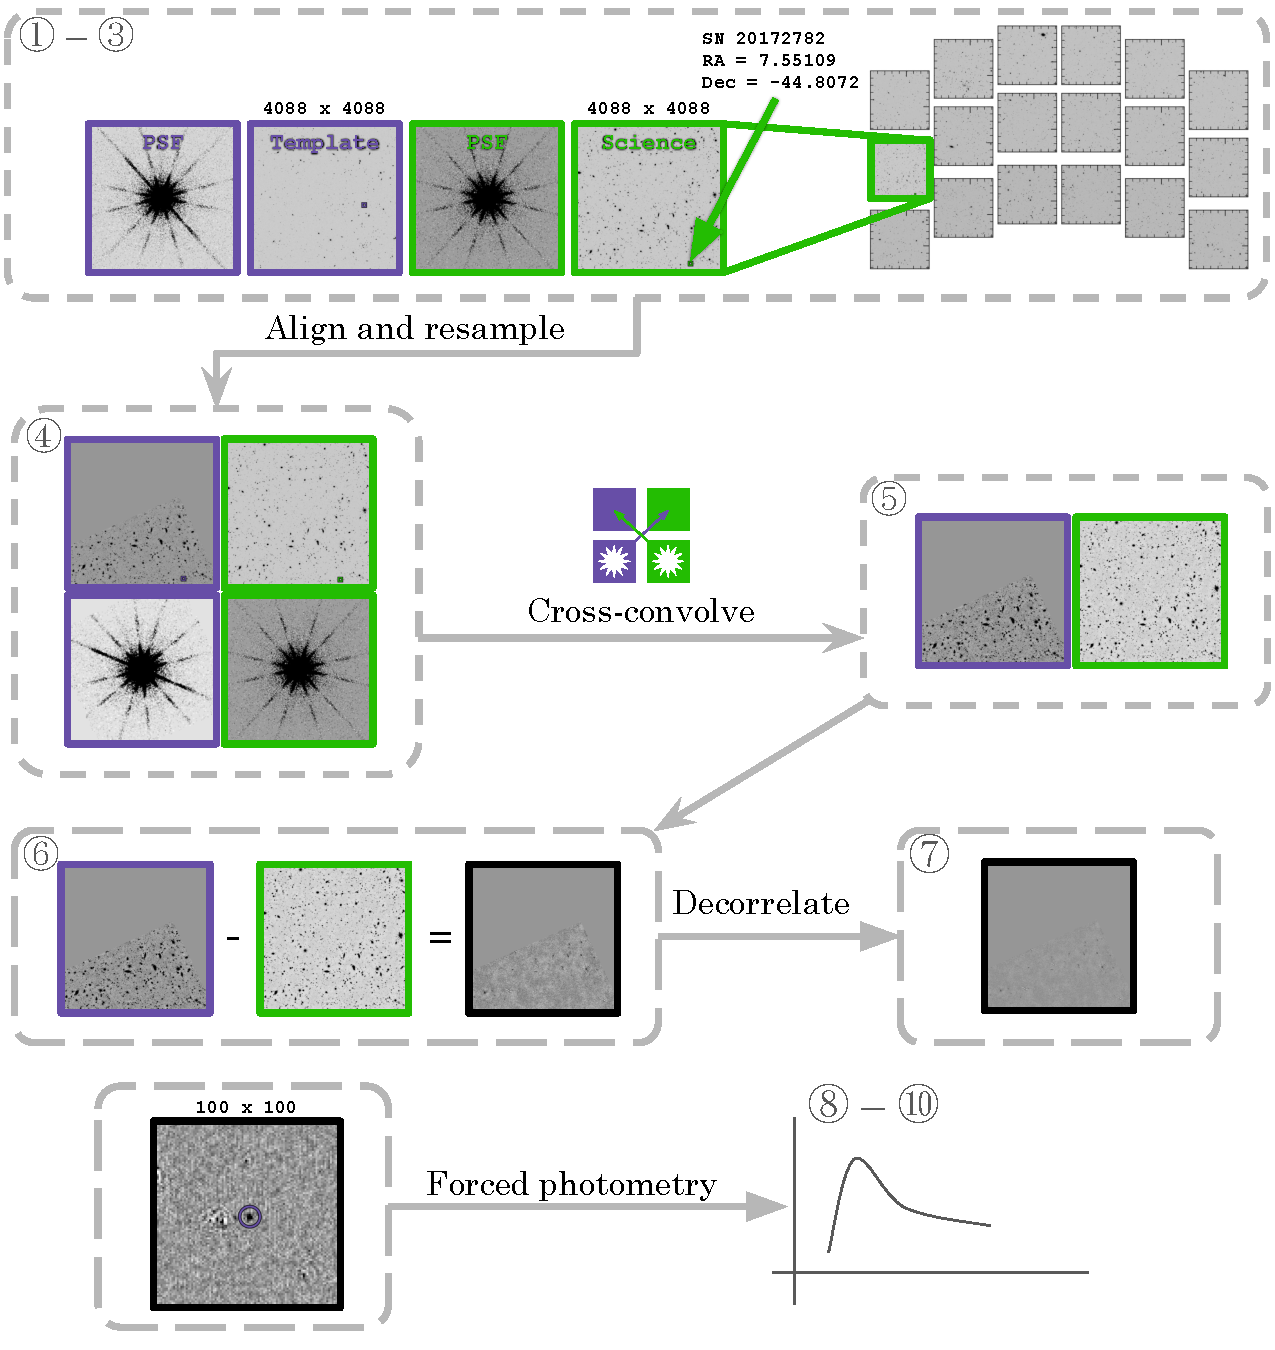
\includegraphics[width=0.99\textwidth]{pipelinefigure.pdf}
   \caption{Visualization of pipeline steps using a sample image from the @openuniverse simulations. Green outlines represent the science image, purple outlines represent the template image, and black outlines represent the difference image. The small inset green and purple squares in panel 1 represent 100 x 100 pixel cutouts.}
   \label{fig:pipeline}
\end{figure}

\begin{figure}
   \centering
   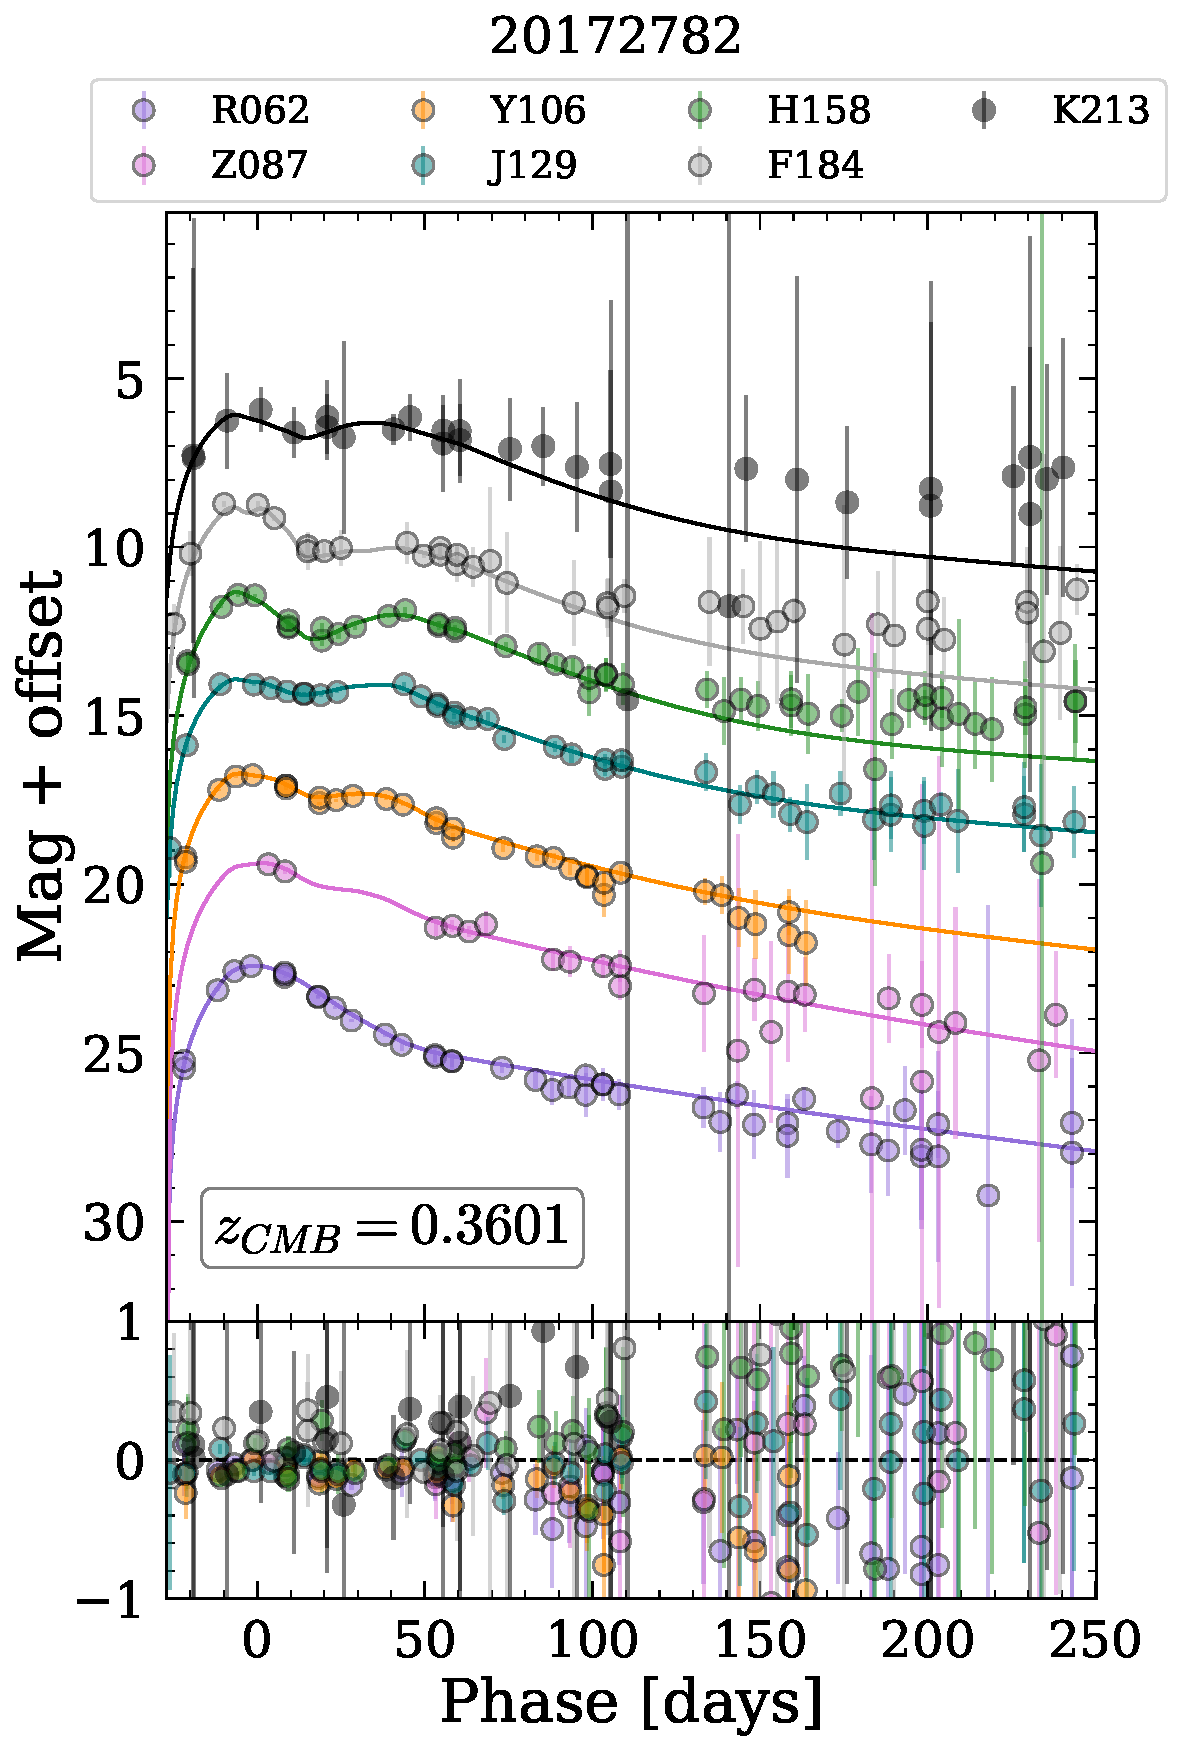
\includegraphics[width=0.5\textwidth]{20172782_lc.pdf}
   \caption{An example light curve, generated using the output of `phrosty`. Circles indicate measured output from `phrosty`, and solid lines are the known simulated light curve from @openuniverse.}
   \label{fig:lc}
\end{figure}

Our pipeline steps are as follows, with ``\texttt{{[}GPU{]}}''
indicating a GPU-accelerated step (Figure \ref{fig:pipeline}):

\begin{enumerate}
\def\labelenumi{\arabic{enumi}.}
\tightlist
\item
  Identify any number of appropriate science (contains SN Ia at a
  specified coordinate) and template images (does not contain SN Ia at
  the same specified coordinate) for a given SN. All input template
  images will be paired with all science images such that if there are
  \(S\) science images and \(T\) template images, the total number of
  difference images is \(S \times T\).
\item
  The pipeline is then called from the command line interface by the
  user. For example,
\end{enumerate}

\begin{verbatim}
SNPIT_CONFIG=phrosty/tests/phrosty_test_config.yaml python phrosty/pipeline.py \
  --oc ou2024 \
  --oid 20172782 \
  -b Y106 \
  --ic ou2024 \
  -t phrosty/tests/20172782_instances_templates_1.csv \
  -s phrosty/tests/20172782_instances_science_2.csv \
  -p 3 -w 3 \
  -v
\end{verbatim}

\texttt{SNPIT\_CONFIG} is the location of a configuration file. The
inputs are: the ``object collection'' associated with the input image
(\texttt{-\/-oc}), the ID number assigned to the object
(\texttt{-\/-oid}), the \emph{Roman} filter matching the data being
processed (\texttt{-b}), the ``image collection'' associated with the
input image (\texttt{-\/-ic}), a list of template images (\texttt{-t}),
a list of science images (\texttt{-s}), the number of parallel CPU
processes for everything except file writing (\texttt{-p}), the number
of parallel CPU process for file writing (\texttt{-w}), and a verbose
flag (\texttt{-v}).

\begin{enumerate}
\def\labelenumi{\arabic{enumi}.}
\setcounter{enumi}{2}
\tightlist
\item
  Subtract the sky background and generate detection masks
  (\citeproc{ref-sourceextractor}{Bertin \& Arnouts, 1996}) for one pair
  of science and template images. Retrieve appropriate PSFs.
\item
  \texttt{{[}GPU{]}} Align the reference image, reference PSF, and
  reference detection mask to the science image.
\item
  \texttt{{[}GPU{]}} Cross-convolve the template PSF with the science
  image, and the science PSF with the template.
\item
  \texttt{{[}GPU{]}} Apply SFFT subtraction (\citeproc{ref-sfft}{Hu et
  al., 2022}) to the cross-convolved images to produce a difference
  image.
\item
  \texttt{{[}GPU{]}} Fit and apply the decorrelation kernel to the
  difference image. Also apply the decorrelation kernel to the science
  PSF and cross-convolved science image to obtain the correct PSF for
  fitting, and the correct image for deriving a zero point from field
  stars for photometry.
\item
  Fit PSF from previous step to field stars in cross-convolved science
  image, cross-match stars to truth catalog, and record median of
  magnitudes for stars with \(19 < m_{truth} < 21.5\) (i.e., not
  saturated and not noisy (\citeproc{ref-aldoroty2025}{Aldoroty et al.,
  2025})).
\item
  Fit the same PSF to the decorrelated difference image at the SN
  coordinates.
\item
  Steps 3--9 are repeated in serial for each science and template image
  pair. Light curve data are collated into a human- and machine-readable
  tabular *.csv file for subsequent analysis. A file is generated for
  each command line call. Thus, each SN has a separate file for each
  filter's data that is processed. These tables are sufficient to plot
  the measured light curve of a SN (Figure \ref{fig:lc}).
\end{enumerate}

Steps 4--7 are part of the SFFT algorithm. The steps that are not
GPU-accelerated, including file writing, are run in parallel processes
on CPUs. The number of parallel processes is controlled by the user.

\section{GPU acceleration and
performance}\label{gpu-acceleration-and-performance}

\label{sec:gpu}

\begin{figure}
   \centering
   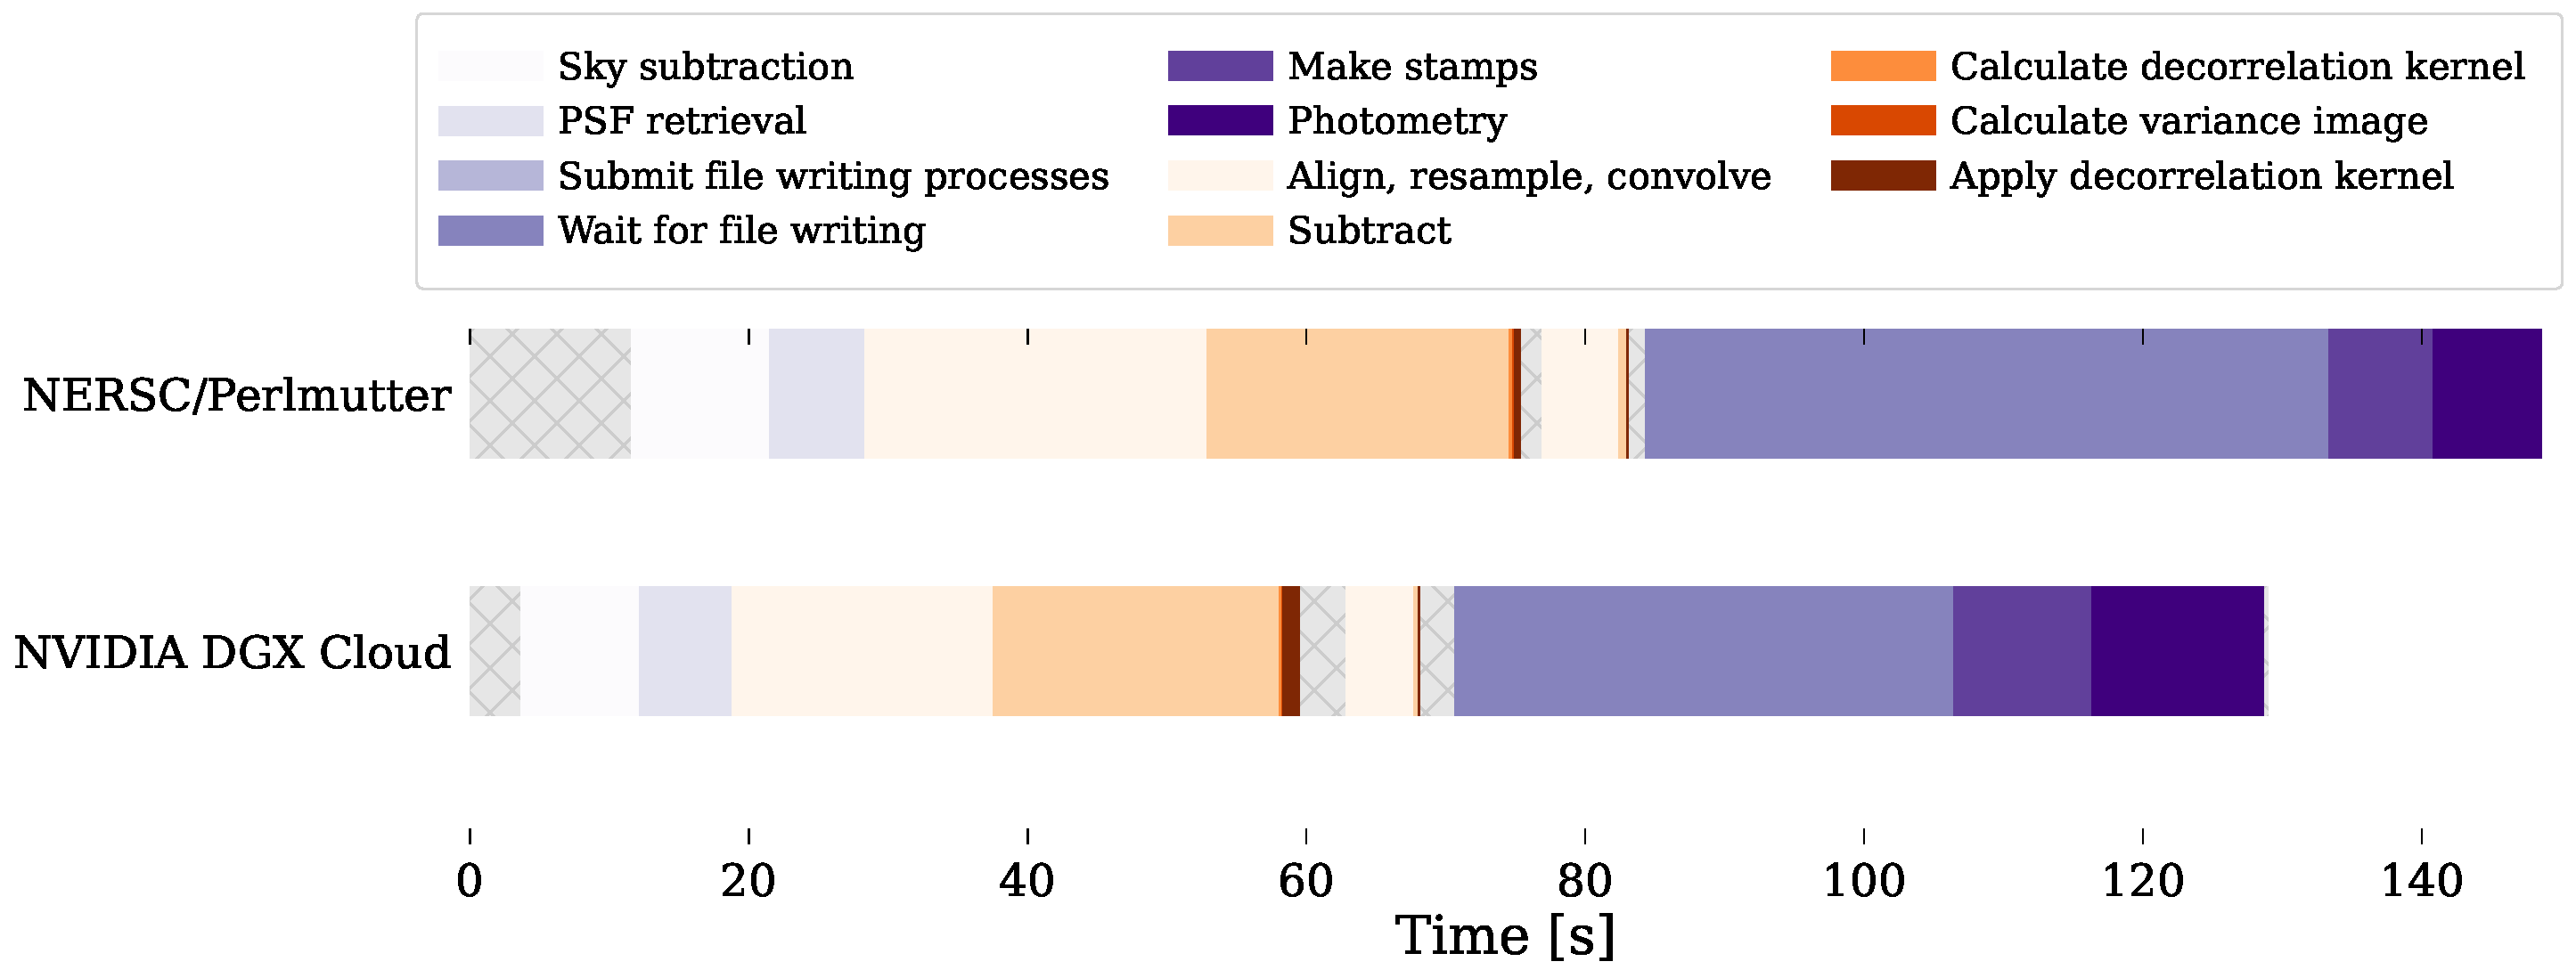
\includegraphics[width=0.99\textwidth]{codeprofiles.pdf}
   \caption{Run times gathered through NVIDIA Nsight Systems profiling for `phrosty`, run on the NVIDIA Curiosity and NERSC Perlmutter clusters. Each profile shows the end-to-end processing of two OpenUniverse images containing SN 20172782. Color bars represent functions in `phrosty`, including calls to external libraries. The grey hatched areas are other computing processes.}
   \label{fig:codeprofile}
\end{figure}

\texttt{phrosty} was developed in part during a hackathon hosted by NASA
and Open Hackathons. During this time, \texttt{phrosty} developers, the
SFFT developer (\citeproc{ref-sfft}{Hu et al., 2022};
\citeproc{ref-sfftjwst}{Hu \& Wang, 2024}), and NVIDIA engineers began
porting more of the original SFFT package to GPU using CUDA
(\citeproc{ref-cuda}{Nickolls et al., 2008}). The final version of SFFT
used by \texttt{phrosty} carries out all matrix operations on GPU, and
holds all data in-memory to minimize time spent on file I/O processes.
In particular, substantial effort was focused on improving image
alignment and resampling code. The NVIDIA Tools Extension SDK (NVTX) is
incorporated throughout the pipeline in order to enable easy code
profiling, which is a unique feature compared to similar software
suites.

\texttt{phrosty} currently runs primarily on NVIDIA A100 GPUs with 40 GB
memory at the National Energy Research Scientific Computing Center's
(NERSC) Perlmutter supercomputer, and has also successfully been run at
the NVIDIA DGX Cluster (Figure \ref{fig:codeprofile}), using one GPU.
When subtracting full \(4088 \times 4088\) images, each SN fully
occupies its GPU's capacity. Thus, the number of SNe that can be run in
parallel is equal to the number of GPUs available. It is possible to
decrease the processed stamp size, in turn decreasing the required
memory and computation time, down to a minimum size of
\(1000\times1000\) px and still obtain high-quality results.

We note that for the first time each GPU function is used (i.e., for the
first image in a batch), there will be additional kernel compilation
overhead time due to \texttt{cupy}'s just-in-time (JIT) compilation.
Subsequent calls are substantially faster; see Figure
\ref{fig:codeprofile} for the run time of a two-image ``light curve''.
Excluding file I/O, the rate-limiting steps are those that rely on
external libraries: sky subtraction
(\citeproc{ref-sourceextractor}{Bertin \& Arnouts, 1996}), PSF model
retrieval, and photometry (\citeproc{ref-photutils}{Bradley et al.,
2024}). All of these processes have been parallelized on CPU. Of these
processes, PSF model retrieval is the most variable. In the case of
cached models, the time to retrieve a PSF is dependent on file I/O.
However, if a model must be generated from a process like photon
shooting (\citeproc{ref-openuniverse}{OpenUniverse et al., 2025}), then
the time to retrieve a PSF can be much longer. Because \texttt{phrosty}
is being developed in advance of the availability of real \emph{Roman}
images, it is compatible with simulations and both of these scenarios
have been run. In the future, PSFs may also be retrieved from STPSF
(\citeproc{ref-stpsf1}{Perrin et al., 2012},
\citeproc{ref-stpsf2}{2014}).

\section{Future development}\label{future-development}

The version of \texttt{phrosty} presented in this work is a prototype.
It will continue to be developed flexibly as \emph{Roman} infrastructure
is added and evolves. Updated versions of \texttt{phrosty} will be
announced in subsequent publications. This includes making the pipeline
fully compatible with \emph{Roman} Science Operations Center (SOC)
products. Currently, compatibility with the
(\citeproc{ref-openuniverse}{OpenUniverse et al., 2025}) simulations is
integrated into the pipeline such that it is reliant on their metadata,
and uses the FITS format versions of all files (where applicable). The
final data products associated with \emph{Roman} will not be FITS
format; the project phases out the FITS file format, and replaces it
with the Advanced Scientific Data Format (ASDF,
(\citeproc{ref-asdf}{Greenfield et al., 2015})). Thus, later versions of
\texttt{phrosty} will be fully compatible with ASDF files.
\texttt{phrosty} will also be kept up-to-date with the latest
calibration data from \emph{Roman}, which we note may necessitate
re-processing of data. This includes, but is not limited to, the PSFs
discussed in Section\textasciitilde{}\ref{sec:gpu} and deeper co-added
templates. These components of the analysis will be crucial in achieving
the required \(<1\%\) flux precision from PSF photometry.

The largest barrier to \texttt{phrosty}'s community accessibility is the
computational resources it requires. Although it is fast (Figure
\ref{fig:codeprofile}), it uses nearly 40 GB of GPU memory for a single
object because fast fourier transforms (FFTs) are inherently
memory-intensive operations due to the large linear system it solves
(\citeproc{ref-sfft}{Hu et al., 2022}). Thus, it requires access to
expensive computing resources, which are not always available to the
entire astronomical community. Although this hardware becomes more
readily available over time as technological advancements continue, and
we do not expect \texttt{phrosty} to ever require more resources than it
demands in its current status, one of our goals for future development
is to reduce \texttt{phrosty}'s memory consumption.

\section{Acknowledgements}\label{acknowledgements}

L. A. thanks Megan Sosey for the discussion about \emph{Roman} HLTDS
data volume.

Funding for the Roman Supernova Project Infrastructure Team has been
provided by NASA under contract to 80NSSC24M0023. This work is also
supported by NASA under award number 80GSFC24M0006. M. T. was funded by
NASA under JPL Contract Task 70-711320, ``Maximizing Science
Exploitation of Simulated Cosmological Survey Data Across Surveys'\,'.

This research used resources of the National Energy Research Scientific
Computing Center, which is supported by the Office of Science of the
U.S. Department of Energy using award number HEP-ERCAP32751.

This work was completed in part at the NASA Open Hackathon, part of the
Open Hackathons program. The authors would like to acknowledge
OpenACC-Standard.org for their support. The authors acknowledge and
thank NVIDIA for their contributions.

\section*{References}\label{references}
\addcontentsline{toc}{section}{References}

\phantomsection\label{refs}
\begin{CSLReferences}{1}{0.5}
\bibitem[\citeproctext]{ref-akeson2019}
Akeson, R., Armus, L., Bachelet, E., Bailey, V., Bartusek, L., Bellini,
A., Benford, D., Bennett, D., Bhattacharya, A., Bohlin, R., Boyer, M.,
Bozza, V., Bryden, G., Calchi Novati, S., Carpenter, K., Casertano, S.,
Choi, A., Content, D., Dayal, P., \ldots{} Zimmerman, N. (2019). {The
Wide Field Infrared Survey Telescope: 100 Hubbles for the 2020s}.
\emph{arXiv e-Prints}, arXiv:1902.05569.
\url{https://doi.org/10.48550/arXiv.1902.05569}

\bibitem[\citeproctext]{ref-aldoroty2025}
Aldoroty, L., Scolnic, D., Kannawadi, A., Knop, R., Rose, B., Hounsell,
R., \& Troxel, M. (2025). {Initial Characterization of Stellar
Photometry of Roman images from the OpenUniverse Simulations}.
\emph{arXiv e-Prints}, arXiv:2506.04332.
\url{https://doi.org/10.48550/arXiv.2506.04332}

\bibitem[\citeproctext]{ref-sourceextractor}
Bertin, E., \& Arnouts, S. (1996). {SExtractor: Software for source
extraction.} \emph{Astronomy and Astrophysics Supplement}, \emph{117},
393--404. \url{https://doi.org/10.1051/aas:1996164}

\bibitem[\citeproctext]{ref-photutils}
Bradley, L., Sipőcz, B., Robitaille, T., Tollerud, E., Vinı́cius, Z.,
Deil, C., Barbary, K., Wilson, T. J., Busko, I., Donath, A., Günther, H.
M., Cara, M., Lim, P. L., Meßlinger, S., Burnett, Z., Conseil, S.,
Droettboom, M., Bostroem, A., Bray, E. M., \ldots{} Perren, G. (2024).
\emph{Astropy/photutils: 1.13.0} (Version 1.13.0). Zenodo.
\url{https://doi.org/10.5281/zenodo.12585239}

\bibitem[\citeproctext]{ref-asdf}
Greenfield, P., Droettboom, M., \& Bray, E. (2015). {ASDF: A new data
format for astronomy}. \emph{Astronomy and Computing}, \emph{12},
240--251. \url{https://doi.org/10.1016/j.ascom.2015.06.004}

\bibitem[\citeproctext]{ref-sfftjwst}
Hu, L., \& Wang, L. (2024). {Differencing and Coadding JWST Images with
Matched Point-spread Function}. \emph{The Astronomical Journal},
\emph{167}(5), 231. \url{https://doi.org/10.3847/1538-3881/ad36cb}

\bibitem[\citeproctext]{ref-sfft}
Hu, L., Wang, L., Chen, X., \& Yang, J. (2022). {Image Subtraction in
Fourier Space}. \emph{The Astrophysical Journal}, \emph{936}(2), 157.
\url{https://doi.org/10.3847/1538-4357/ac7394}

\bibitem[\citeproctext]{ref-kessler2015}
Kessler, R., Marriner, J., Childress, M., Covarrubias, R., D'Andrea, C.
B., Finley, D. A., Fischer, J., Foley, R. J., Goldstein, D., Gupta, R.
R., Kuehn, K., Marcha, M., Nichol, R. C., Papadopoulos, A., Sako, M.,
Scolnic, D., Smith, M., Sullivan, M., Wester, W., \ldots{} DES
Collaboration. (2015). {The Difference Imaging Pipeline for the
Transient Search in the Dark Energy Survey}. \emph{150}(6), 172.
\url{https://doi.org/10.1088/0004-6256/150/6/172}

\bibitem[\citeproctext]{ref-cuda}
Nickolls, J., Buck, I., Garland, M., \& Skadron, K. (2008). Scalable
parallel programming with CUDA: Is CUDA the parallel programming model
that application developers have been waiting for? \emph{Queue},
\emph{6}(2), 40--53. \url{https://doi.org/10.1145/1365490.1365500}

\bibitem[\citeproctext]{ref-rotacreport}
Observations Time Allocation Committee, R., \& Community Survey
Definition Committees, C. (2025). {Roman Observations Time Allocation
Committee: Final Report and Recommendations}. \emph{arXiv e-Prints},
arXiv:2505.10574. \url{https://doi.org/10.48550/arXiv.2505.10574}

\bibitem[\citeproctext]{ref-openuniverse}
OpenUniverse, The LSST Dark Energy Science Collaboration, The Roman HLIS
Project Infrastructure Team, The Roman RAPID Project Infrastructure
Team, The Roman Supernova Cosmology Project Infrastructure Team,
Alarcon, A., Aldoroty, L., Beltz-Mohrmann, G., Bera, A., Blazek, J.,
Bogart, J., Braeunlich, G., Broughton, A., Cao, K., Chiang, J., Chisari,
N. E., Desai, V., Fang, Y., Galbany, L., \ldots{} Zhang, T. (2025).
{OpenUniverse2024: A shared, simulated view of the sky for the next
generation of cosmological surveys}. \emph{arXiv e-Prints},
arXiv:2501.05632. \url{https://doi.org/10.48550/arXiv.2501.05632}

\bibitem[\citeproctext]{ref-stpsf2}
Perrin, M. D., Sivaramakrishnan, A., Lajoie, C.-P., Elliott, E., Pueyo,
L., Ravindranath, S., \& Albert, Loı̈c. (2014). {Updated point spread
function simulations for JWST with WebbPSF}. In J. M. Oschmann Jr., M.
Clampin, G. G. Fazio, \& H. A. MacEwen (Eds.), \emph{Space telescopes
and instrumentation 2014: Optical, infrared, and millimeter wave} (Vol.
9143, p. 91433X). \url{https://doi.org/10.1117/12.2056689}

\bibitem[\citeproctext]{ref-stpsf1}
Perrin, M. D., Soummer, R., Elliott, E. M., Lallo, M. D., \&
Sivaramakrishnan, A. (2012). {Simulating point spread functions for the
James Webb Space Telescope with WebbPSF}. In M. C. Clampin, G. G. Fazio,
H. A. MacEwen, \& J. M. Oschmann Jr. (Eds.), \emph{Space telescopes and
instrumentation 2012: Optical, infrared, and millimeter wave} (Vol.
8442, p. 84423D). \url{https://doi.org/10.1117/12.925230}

\bibitem[\citeproctext]{ref-spergel2015}
Spergel, D., Gehrels, N., Baltay, C., Bennett, D., Breckinridge, J.,
Donahue, M., Dressler, A., Gaudi, B. S., Greene, T., Guyon, O., Hirata,
C., Kalirai, J., Kasdin, N. J., Macintosh, B., Moos, W., Perlmutter, S.,
Postman, M., Rauscher, B., Rhodes, J., \ldots{} Zhao, F. (2015).
{Wide-Field InfrarRed Survey Telescope-Astrophysics Focused Telescope
Assets WFIRST-AFTA 2015 Report}. \emph{arXiv e-Prints},
arXiv:1503.03757. \url{https://doi.org/10.48550/arXiv.1503.03757}

\bibitem[\citeproctext]{ref-spergel2013}
Spergel, D., Gehrels, N., Breckinridge, J., Donahue, M., Dressler, A.,
Gaudi, B. S., Greene, T., Guyon, O., Hirata, C., Kalirai, J., Kasdin, N.
J., Moos, W., Perlmutter, S., Postman, M., Rauscher, B., Rhodes, J.,
Wang, Y., Weinberg, D., Centrella, J., \ldots{} Shaklan, S. (2013).
{WFIRST-2.4: What Every Astronomer Should Know}. \emph{arXiv e-Prints},
arXiv:1305.5425. \url{https://doi.org/10.48550/arXiv.1305.5425}

\end{CSLReferences}

\end{document}
